\documentclass[12pt,a4paper]{report}

% ── Packages ──────────────────────────────────────────────────────────────────
\usepackage[T1]{fontenc}
\usepackage[utf8]{inputenc}
\usepackage[english]{babel}
\usepackage{geometry}
\usepackage{graphicx}
\usepackage{hyperref}
\usepackage{fancyhdr}
\usepackage{titlesec}
\usepackage{setspace}
\usepackage{parskip}
\usepackage{xcolor}
\usepackage{booktabs}
\usepackage{array}
\usepackage{longtable}
\usepackage{tabularx}
\usepackage{colortbl}
\usepackage{enumitem}
\usepackage{emptypage}
\usepackage{float}
\usepackage{caption}
\usepackage{mdframed}
\usepackage{amsmath}
\usepackage{afterpage}
\usepackage{tikz}
\usepackage{tcolorbox}
\tcbuselibrary{skins,breakable}
\usetikzlibrary{shapes.geometric,positioning}

% ── Geometry ──────────────────────────────────────────────────────────────────
\geometry{a4paper, top=2.5cm, bottom=2.5cm, left=3cm, right=2.5cm, headheight=15pt}

% ── Colours ───────────────────────────────────────────────────────────────────
\definecolor{b2ablue}{RGB}{30,80,150}
\definecolor{accentgray}{RGB}{90,90,90}
\definecolor{placeholderbg}{RGB}{255,250,230}
\definecolor{placeholderborder}{RGB}{200,160,0}
\definecolor{screenshotbg}{RGB}{240,248,255}
\definecolor{screenshotborder}{RGB}{100,149,237}
\definecolor{logobg}{RGB}{235,235,235}
\definecolor{logoborder}{RGB}{180,180,180}
% Architecture diagram colours
\definecolor{layerfront}{RGB}{219,234,254}
\definecolor{layerback}{RGB}{220,252,231}
\definecolor{layerml}{RGB}{254,243,199}
\definecolor{layerdb}{RGB}{243,232,255}
\definecolor{layerinfra}{RGB}{255,228,230}
\definecolor{arrowcol}{RGB}{100,116,139}

% ── Hyperref ──────────────────────────────────────────────────────────────────
\hypersetup{colorlinks=true,linkcolor=b2ablue,urlcolor=b2ablue,citecolor=b2ablue,
  pdftitle={B2A Smart-Resource PFE},pdfauthor={Othmen Khedhri}}

% ── Spacing ───────────────────────────────────────────────────────────────────
\onehalfspacing
\setlist[itemize]{noitemsep, topsep=4pt}
\setlist[enumerate]{noitemsep, topsep=4pt}

% ── Chapter / section styles ──────────────────────────────────────────────────
\titleformat{\chapter}[display]{\normalfont\bfseries\Large\color{b2ablue}}
  {\chaptertitlename\ \thechapter}{10pt}{\huge}
\titlespacing*{\chapter}{0pt}{20pt}{12pt}
\titleformat{\section}{\normalfont\bfseries\large\color{b2ablue}}{\thesection}{1em}{}
\titlespacing*{\section}{0pt}{10pt}{4pt}
\titleformat{\subsection}{\normalfont\bfseries\normalsize\color{accentgray}}{\thesubsection}{1em}{}
\titlespacing*{\subsection}{0pt}{8pt}{2pt}

% ── Header / footer ───────────────────────────────────────────────────────────
\pagestyle{fancy}\fancyhf{}
\fancyhead[L]{\small\textcolor{accentgray}{B2A Smart-Resource --- PFE}}
\fancyhead[R]{\small\textcolor{accentgray}{\leftmark}}
\fancyfoot[C]{\small\thepage}
\renewcommand{\headrulewidth}{0.4pt}

% ── Diagram placeholder ───────────────────────────────────────────────────────
\newmdenv[backgroundcolor=placeholderbg,linecolor=placeholderborder,
  linewidth=1pt,innerleftmargin=8pt,innerrightmargin=8pt,
  innertopmargin=6pt,innerbottommargin=6pt,roundcorner=3pt]{placeholder}
\newcommand{\ssd}[1]{\begin{placeholder}\textbf{[SSD --- #1]}\end{placeholder}\vspace{2pt}}
\newcommand{\sod}[1]{\begin{placeholder}\textbf{[SOD --- #1]}\end{placeholder}\vspace{4pt}}

% ── Screenshot annex reference ────────────────────────────────────────────────
\newmdenv[backgroundcolor=screenshotbg,linecolor=screenshotborder,
  linewidth=0.8pt,innerleftmargin=8pt,innerrightmargin=8pt,
  innertopmargin=5pt,innerbottommargin=5pt,roundcorner=3pt]{screenshotbox}
\newcommand{\annexref}[1]{\begin{screenshotbox}\small\textit{Screenshots for \textbf{#1} are in the Appendix, p.\,\pageref{annex:#1}.}\end{screenshotbox}\vspace{4pt}}

% ── Logo placeholder (inline, fixed size) ────────────────────────────────────
\newcommand{\logoplace}[1]{%
  \begin{tikzpicture}[baseline=-0.5ex]
    \node[fill=logobg, draw=logoborder, rounded corners=4pt,
          inner xsep=6pt, inner ysep=4pt,
          minimum width=2.4cm, minimum height=0.75cm,
          font=\bfseries\footnotesize\color{accentgray}] {#1};
  \end{tikzpicture}%
}

% ── Tech table with logo column ───────────────────────────────────────────────
\newenvironment{techtable}[2]{%
  \begin{longtable}{>{\centering\arraybackslash}p{2.6cm} p{11cm}}
  \caption{#1}\label{#2}\\
  \toprule\textbf{Technology} & \textbf{Role in this Chapter}\\\midrule\endhead
  \midrule\multicolumn{2}{r}{\small\itshape Continued\ldots}\\\endfoot
  \bottomrule\endlastfoot
}{%
  \end{longtable}%
}

% ── Compact layer badge for architecture overview ─────────────────────────────
\newcommand{\layerbadge}[2]{%
  \begin{tikzpicture}[baseline=-0.5ex]
    \node[fill=#1, rounded corners=3pt,
          inner xsep=5pt, inner ysep=3pt,
          font=\bfseries\scriptsize\color{b2ablue}] {#2};
  \end{tikzpicture}%
}

% ── TOC depth ─────────────────────────────────────────────────────────────────
\setcounter{tocdepth}{1}
\setcounter{secnumdepth}{3}

% ══════════════════════════════════════════════════════════════════════════════
\begin{document}

% ── Title page ────────────────────────────────────────────────────────────────
\begin{titlepage}\centering
  \vspace*{1cm}
  {\Large\bfseries\color{b2ablue}
    Republic of Tunisia\\[3pt]
    Ministry of Higher Education and Scientific Research}\\[0.4cm]
  \rule{\linewidth}{1.5pt}\\[0.3cm]
  {\large\itshape University of \rule{5cm}{0.4pt}}\\[0.2cm]
  {\large\itshape Faculty / Higher Institute of \rule{4cm}{0.4pt}}\\[0.9cm]
  {\Huge\bfseries\color{b2ablue} B2A Smart-Resource}\\[0.35cm]
  {\Large\bfseries A Smart Full-Stack Resource Management Platform\\
   for an Accounting and Consulting Firm}\\[0.7cm]
  \rule{\linewidth}{0.8pt}\\[0.6cm]
  {\large Final Year Project Report (PFE)\\
   Submitted in Partial Fulfillment of the Requirements for the\\
   \textbf{Licence Degree (L3) in Computer Science}}\\[0.9cm]
  \begin{tabular}{rl}
    \textbf{Authors:}       & Othmen Khedhri \& \rule{4cm}{0.4pt}\\[4pt]
    \textbf{Supervisor:}    & \rule{6cm}{0.4pt}\\[4pt]
    \textbf{Host Company:}  & B2A Accounting \& Consulting Firm\\[4pt]
    \textbf{Academic Year:} & 2024--2025\\
  \end{tabular}\\[1.5cm]
  \vfill\rule{\linewidth}{1.5pt}
\end{titlepage}

% ── Front matter ──────────────────────────────────────────────────────────────
\pagenumbering{roman}\setcounter{page}{2}

\chapter*{Dedication}\addcontentsline{toc}{chapter}{Dedication}\thispagestyle{plain}
\begin{center}\vspace*{1.5cm}
{\itshape To our families, whose patience and encouragement carried us through the long nights.\\[0.4em]
 To our professors, whose standards pushed us further than we thought possible.\\[0.4em]
 To the entire team at B2A, who trusted two students with a real problem
 and gave us the freedom to solve it properly.}
\end{center}

\chapter*{Acknowledgements}\addcontentsline{toc}{chapter}{Acknowledgements}\thispagestyle{plain}
Our deepest thanks go to the B2A management team for the quality of their involvement.
Rather than handing us a vague brief, they shared their actual day-to-day frustrations ---
the hours spent consolidating spreadsheets, the guesswork in estimating mission budgets,
the inability to spot a drifting client relationship before it became a problem.
Those conversations were the real specification document of this project.

To our academic supervisor: thank you for the rigour.
To the open-source communities behind React, Node.js, FastAPI, and MongoDB:
the quality of your documentation made a difference every single day.

\chapter*{Abstract}\addcontentsline{toc}{chapter}{Abstract}\thispagestyle{plain}
This report describes \textit{B2A Smart-Resource}, a full-stack web platform developed
during a final-year internship at B2A, a Tunisian accounting and consulting firm.
The platform replaces a collection of manually maintained Excel files and informal
workflows with a unified, multi-role application covering staff management, client
and project tracking, timesheet ingestion, pace monitoring, ML-powered budget estimation,
and an immutable audit trail.

The frontend is a React~19 single-page application built with Vite and fully typed
in TypeScript. The backend is a Node.js~20 / Express~5 REST API, also in TypeScript,
connected to MongoDB Atlas through Mongoose. A Python~3.11 FastAPI microservice,
auto-spawned at server startup, handles machine learning predictions using trained
gradient-boosting regression models.

\textbf{Keywords:} resource management, full-stack, React, Node.js, FastAPI, machine
learning, MongoDB, audit trail, pace index, TypeScript, Scrum.

\tableofcontents\addcontentsline{toc}{chapter}{Table of Contents}
\listoftables\addcontentsline{toc}{chapter}{List of Tables}

\chapter*{List of Acronyms}\addcontentsline{toc}{chapter}{List of Acronyms}\thispagestyle{plain}
\begin{longtable}{>{\bfseries}p{3cm} p{10.5cm}}
  \toprule Acronym & Meaning\\\midrule\endhead
  API   & Application Programming Interface\\
  ASGI  & Asynchronous Server Gateway Interface\\
  JWT   & JSON Web Token\\
  KNN   & K-Nearest Neighbours\\
  KPI   & Key Performance Indicator\\
  MAE   & Mean Absolute Error\\
  ML    & Machine Learning\\
  ODM   & Object Document Mapper\\
  PFE   & Projet de Fin d\'Etudes (Final Year Project)\\
  RBAC  & Role-Based Access Control\\
  REST  & Representational State Transfer\\
  SPA   & Single-Page Application\\
  SSD   & System Sequence Diagram\\
  SOD   & Sequence Object Diagram\\
  TND   & Tunisian Dinar\\
  TTL   & Time To Live\\
  VPS   & Virtual Private Server\\
  \bottomrule
\end{longtable}

% ── Main matter ───────────────────────────────────────────────────────────────
\cleardoublepage\pagenumbering{arabic}\setcounter{page}{1}

% ══════════════════════════════════════════════════════════════════════════════
% CHAPTER 1 — General Context
% ══════════════════════════════════════════════════════════════════════════════
\chapter{General Context and Project Presentation}

\section{Host Organisation and Problem Statement}

Walk into any mid-sized accounting firm on a busy Monday morning and you will find a
familiar scene: someone has just emailed a spreadsheet to three colleagues asking them
to fill in their hours for last month. Someone else is piecing together a budget
proposal for a new client using figures recalled from a mission two years back. A
partner is trying to determine whether a long-running engagement is still profitable,
armed with nothing but a printout and a highlighter. This is not a caricature --- it
is exactly what we found at B2A.

B2A is a Tunisian accounting and consulting firm delivering statutory auditing, tax
advisory, payroll management, and business consulting. Every client engagement is
structured as one or more missions, each with a defined scope, a budget in hours, a
contract value in TND, and a team of collaborators responsible for delivering it.
The firm is well-run and its people are skilled. The problem was never competence
--- it was infrastructure.

Our requirement interviews surfaced five concrete, recurring frustrations that no
amount of spreadsheet discipline could permanently solve:

\begin{itemize}
  \item \textbf{No real-time budget visibility} --- consumption figures were only
        known after a monthly manual consolidation that took hours and was already
        stale by the time it reached the partner's desk.
  \item \textbf{Workload blind spots} --- there was no reliable way to see a
        collaborator's true load across all active missions at once. Burnout crept
        up quietly and was noticed too late.
  \item \textbf{No pace monitoring} --- whether an annual client contract was
        drifting off-track was tracked informally at best, and corrected too late
        at worst.
  \item \textbf{Evidence-free estimation} --- budget proposals for new missions
        relied entirely on personal memory and gut feel. There was no structured
        access to what similar past missions had actually cost.
  \item \textbf{No audit trail} --- no record existed of who changed what and when.
        In a firm where compliance is the core product, this was a glaring gap.
\end{itemize}

Each problem had a workaround. None of the workarounds scaled.

\section{Proposed Solution}

\textit{B2A Smart-Resource} is a single unified web platform that replaces every
spreadsheet and manual workflow the firm relied on.

It covers: staff and HR management with live workload and burnout detection; client
and project tracking with real-time budget consumption; a collaborator--client hours
heatmap; a server-side file parser; monthly timesheet upload and tracking; annual
budget import; a client-level pace index with year-end TND projection; an ML-powered
budget estimator trained on real historical data; a team builder; an immutable audit
trail; and a bilingual help guide in English and French.

Every feature on that list was asked for by name.

\section{Development Methodology}

\textbf{Agile} \logoplace{Agile} is a development philosophy: build in short cycles,
show real results, adjust based on feedback. No long plans that reality will break.

We used \textbf{Scrum} \logoplace{Scrum} as our Agile framework --- the right choice
for this project because B2A's requirements were clear on the \textit{problems} but
not always on the exact \textit{solutions}. Five two-week sprints with a stakeholder
review at the end of each one meant corrections happened early, not after months of
wrong-direction work.

Two examples that prove the point: column totals on the heatmap were added after a
Sprint~2 demo. The year-end TND profit projection came from a partner who said during
Sprint~4: \textit{``I don't just want to know where I am. I want to know where I'll
end up.''} Neither was in the original specification.

\section{Product Backlog}

Before any code was written, the full scope of the platform was formalised as a
prioritised product backlog. Each user story was assigned a priority, an effort
estimate in story points, and a target sprint. The complete backlog is presented
below --- it gives the reader an immediate and complete picture of what was built,
for whom, and in what order.

\begin{longtable}{>{\bfseries}p{1.1cm} p{6.8cm} >{\centering\arraybackslash}p{1.6cm}
                  >{\centering\arraybackslash}p{1.4cm} >{\centering\arraybackslash}p{1.2cm}}
  \caption{Product Backlog --- B2A Smart-Resource}\label{tab:backlog}\\
  \toprule
  \textbf{ID} & \textbf{User Story} & \textbf{Priority} & \textbf{Points} & \textbf{Sprint}\\
  \midrule\endhead
  \midrule\multicolumn{5}{r}{\small\itshape Continued\ldots}\\\endfoot
  \bottomrule\endlastfoot

  US01 & As an Admin, I want to log in securely so that only authorised users access the platform.
        & High & 5 & S1\\[3pt]
  US02 & As an Admin, I want my session to expire after inactivity so that my data stays protected.
        & High & 3 & S1\\[3pt]
  US03 & As an Admin, I want to be logged out across all tabs simultaneously so that no active session is left unattended.
        & Medium & 3 & S1\\[3pt]
  US04 & As an Admin, I want a comprehensive dashboard so that I can monitor the firm's operational health at a glance.
        & High & 13 & S1\\[3pt]
  US05 & As an Admin, I want in-app notifications so that I am alerted to critical situations without checking every module.
        & Medium & 5 & S1\\[3pt]
  US06 & As an Admin, I want a bilingual help guide so that I can find answers without leaving the platform.
        & Low & 3 & S1\\[3pt]
  US07 & As an Admin, I want to manage staff profiles with real-time workload data so that I can detect burnout risk early.
        & High & 8 & S2\\[3pt]
  US08 & As an Admin, I want to manage client records with full legal metadata so that all client information is centralised.
        & High & 5 & S2\\[3pt]
  US09 & As an Admin, I want to track project budgets in real time so that I can act before a budget is exceeded.
        & High & 8 & S2\\[3pt]
  US10 & As an Admin, I want a collaborator--client hours heatmap so that I can spot workload imbalances instantly.
        & Medium & 5 & S2\\[3pt]
  US11 & As an Admin, I want to parse and clean raw Excel files in the platform so that I no longer depend on local scripts.
        & High & 8 & S3\\[3pt]
  US12 & As an Admin, I want to import timesheets, annual budgets, and leave records so that all operational data is centralised and validated automatically.
        & High & 13 & S3\\[3pt]
  US13 & As an Admin, I want to monitor budget consumption at both project and client level with year-end projections so that I can anticipate overruns before they happen.
        & High & 13 & S4\\[3pt]
  US14 & As an Admin, I want ML-powered budget estimates with confidence levels so that mission proposals are evidence-based.
        & High & 13 & S4\\[3pt]
  US15 & As an Admin, I want to build mission teams with live cost and experience summaries so that staffing decisions are informed.
        & Medium & 8 & S4\\[3pt]
  US16 & As a Super Admin, I want to create and delete Admin accounts so that platform access is fully controlled.
        & High & 5 & S5\\[3pt]
  US17 & As a Super Admin, I want an immutable audit trail with field-level diffs so that every action on the platform is traceable.
        & High & 8 & S5\\[3pt]
  US18 & As an Admin, I want the platform deployed with zero-downtime updates so that operations are never interrupted.
        & Medium & 5 & S5\\[3pt]

\end{longtable}

Eighteen user stories totalling 133 story points across five sprints. The effort
distribution is deliberately front-loaded: the highest-complexity stories --- the
dashboard (13 points), the import pipeline (13 points), the pace index (13 points),
and the ML estimator (13 points) --- were identified early and placed into sprints
where their data dependencies would already be satisfied.

\begin{longtable}{>{\bfseries}p{1.6cm} p{3cm} p{4.8cm} p{3.4cm}}
  \caption{Five-Sprint Project Plan with User Stories}\label{tab:sprints}\\
  \toprule
  \textbf{Sprint} & \textbf{Domain} & \textbf{Key Deliverables} & \textbf{Stories}\\
  \midrule\endhead
  \midrule\multicolumn{4}{r}{\small\itshape Continued\ldots}\\\endfoot
  \bottomrule\endlastfoot

  Sprint 1 & Identity \& Visibility
            & Secure login, inactivity timeout, cross-tab logout, nine-section dashboard, notification bell, bilingual help guide
            & US01, US02, US03, US04, US05, US06\\[6pt]

  Sprint 2 & Core Resource Management
            & Staff profiles with workload tracking and burnout detection, client directory with legal metadata, real-time project budget monitoring, collaborator--client hours heatmap
            & US07, US08, US09, US10\\[6pt]

  Sprint 3 & Data Ingestion
            & Server-side file parser, monthly timesheet upload and tracking, Excel import pipeline (time entries, billing, leave), annual budget import
            & US11, US12\\[6pt]

  Sprint 4 & Intelligence \& Analytics
            & Client-level pace index with year-end TND projection, ML-powered budget estimator with three-point confidence output, team builder with live cost summary
            & US13, US14, US15\\[6pt]

  Sprint 5 & Governance \& Deployment
            & Admin account management, immutable audit trail with field-level diffs and CSV export, production infrastructure with zero-downtime CI/CD pipeline
            & US16, US17, US18\\[6pt]

\end{longtable}

\section{Overall Architecture}

The platform is built around four components: a React frontend, a Node.js backend,
a Python ML microservice, and a MongoDB Atlas database. The full architecture diagram
and the reasoning behind each component are detailed in Chapter~\ref{chap:arch}.

% ══════════════════════════════════════════════════════════════════════════════
% CHAPTER 2 — Requirements Analysis
% ══════════════════════════════════════════════════════════════════════════════
\chapter{Requirements Analysis}

\section{Actors and Permissions}

\begin{longtable}{>{\bfseries}p{2.8cm} p{10.7cm}}
  \caption{Actor Permissions}\label{tab:actors}\\
  \toprule Role & Permissions\\\midrule\endhead
  Super Admin  & Unrestricted access to every module in the system: user management, orphan data cleanup, full audit trail with CSV export, all deletions, ML retrain trigger, and all configuration settings. The only role that can create or deactivate other administrators.\\
  Admin        & Full operational access: projects, clients, staff, assignments, timesheets, file parser, all Excel imports, annual budgets, leave management, and analytics. Cannot manage other administrators or access platform-level configuration reserved for the Super Admin.\\
  \bottomrule
\end{longtable}

\section{Functional Requirements}

The platform covers fifteen functional areas: multi-role authentication with brute-force protection and cross-tab session sync; a nine-section role-aware dashboard; staff management with workload and burnout detection; client management with legal metadata and bulk import; project management with pace tracking and threshold alerts; a collaborator--client hours heatmap built from timesheets; a server-side file parser replacing two Python scripts; monthly timesheet upload and tracking; annual budget import per client; leave CRUD; a client-level pace index with year-end projection and TND profit prediction; an ML budget estimator with three-point estimates and similar project references; a team builder for staffing decisions; an immutable 365-day audit trail with field-level diffs and CSV export; and a bilingual in-app help guide.

\section{Non-Functional Requirements}

\begin{longtable}{>{\bfseries}p{3.2cm} p{10.3cm}}
  \caption{Non-Functional Requirements}\label{tab:nfr}\\
  \toprule Attribute & Requirement\\\midrule\endhead
  Security        & All endpoints protected by JWT; RBAC middleware on every route; brute-force and token blacklisting active.\\
  Performance     & Standard queries $\leq$ 500\,ms; dashboard data in a single aggregated payload; lazy-loaded pages.\\
  Usability       & Full EN/FR bilingual interface with 200+ translation keys; precise actionable error messages.\\
  Reliability     & Failed imports report exact failing rows; orphan cleanup utility for data consistency.\\
  Auditability    & Every state-change logged with actor, timestamp, IP, user agent, and field-level diff; 365-day TTL; CSV export.\\
  Maintainability & Full TypeScript on both frontend and backend; ML auto-retrains at 10 new completions.\\
  \bottomrule
\end{longtable}

\section{Global Use Case Diagram}
\begin{placeholder}\textbf{[Use Case Diagram --- Global System: to be inserted here]}\end{placeholder}

\section{Requirements Specification with UML}

\textbf{UML} \logoplace{UML} (Unified Modelling Language) was used to model the
system before and during development. With four components communicating across the
platform, diagrams were the fastest way to align the team and validate with B2A
stakeholders without asking them to read code.

Two diagram types are used throughout this report:

\begin{itemize}
  \item \textbf{SSD (System Sequence Diagram)} --- shows the order of interactions
        between the user and the system for a given feature.
  \item \textbf{SOD (Sequence Object Diagram)} --- shows how the internal components
        (frontend, backend, database, ML service) communicate to fulfil a request.
\end{itemize}

Each sprint chapter includes both diagrams for every feature it introduces.

% ══════════════════════════════════════════════════════════════════════════════
% CHAPTER 3 — System Architecture & Technology Blueprint
% ══════════════════════════════════════════════════════════════════════════════
\chapter{System Architecture and Technology                              
Blueprint}
\label{chap:arch}

Rather than cataloguing every library upfront, this chapter presents the platform as a
coherent architecture and explains the reasoning behind each structural decision.
Specific technologies are detailed within the sprint chapter where they are actually put to work.

\section{Architectural Overview}

B2A Smart-Resource follows a \textbf{three-tier, four-component} architecture designed
to keep each concern completely isolated: the browser never speaks directly to the
database; the ML microservice is never exposed to the public internet; the deployment
stack mirrors the development stack to eliminate environment drift.

\vspace{0.8em}

% ── Architecture diagram (simple, jury-friendly) ──────────────────────────────
\begin{center}
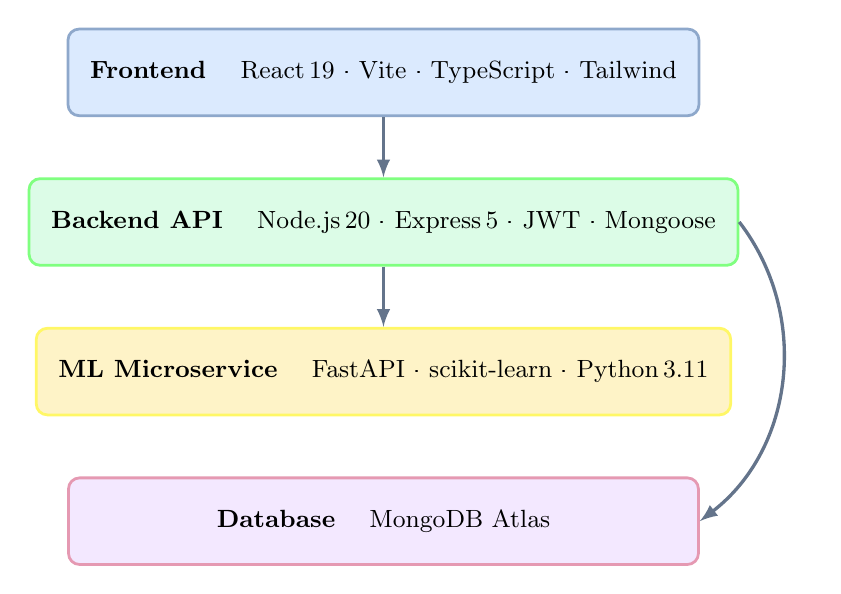
\begin{tikzpicture}[
  font=\small,
  box/.style={rounded corners=4pt, minimum width=8cm, minimum height=1.1cm,
              draw, line width=1pt, align=center, inner sep=8pt},
  arr/.style={-latex, line width=1.2pt, color=arrowcol}
]

\node[box, fill=layerfront,  draw=b2ablue!50] (spa)   at (0, 0)    {\textbf{Frontend} \quad React\,19 · Vite · TypeScript · Tailwind};
\node[box, fill=layerback,   draw=green!50]   (api)   at (0,-1.9)  {\textbf{Backend API} \quad Node.js\,20 · Express\,5 · JWT · Mongoose};
\node[box, fill=layerml,     draw=yellow!60]  (ml)    at (0,-3.8)  {\textbf{ML Microservice} \quad FastAPI · scikit-learn · Python\,3.11};
\node[box, fill=layerdb,     draw=purple!40]  (db)    at (0,-5.7)  {\textbf{Database} \quad MongoDB Atlas};

\draw[arr] (spa.south) -- (api.north);
\draw[arr] (api.south) -- (ml.north);
\draw[arr, bend left=45] (api.east) to (db.east);

\end{tikzpicture}

\smallskip
{\small\textit{Figure: B2A Smart-Resource --- Four-Component Architecture}}
\end{center}

\vspace{0.6em}

\section{Technology Selection Rationale}

Each technology was chosen for a single practical reason.

\begin{longtable}{>{\bfseries}p{3.5cm} p{10cm}}
  \caption{Technology Choices and Reasoning}\label{tab:rationale}\\
  \toprule \textbf{Technology} & \textbf{Why}\\\midrule\endhead
  \midrule\multicolumn{2}{r}{\small\itshape Continued\ldots}\\\endfoot
  \bottomrule\endlastfoot

  React 19 + TypeScript  & Component model fits a multi-section dashboard; TypeScript catches errors before they reach production.\\[4pt]
  Vite 7                 & Dev proxy matches the production Nginx setup exactly --- no routing surprises when deploying.\\[4pt]
  Tailwind CSS 4         & Utility classes make theming and dark mode trivial without a separate CSS file.\\[4pt]
  Node.js 20 / Express 5 & Same language as the frontend (TypeScript); async by default; large ecosystem for every utility needed.\\[4pt]
  MongoDB Atlas          & Document model fits variable mission structures naturally; Atlas handles backups and scaling out of the box.\\[4pt]
  Mongoose               & Schema validation on top of MongoDB; enforces data integrity without a separate migration system.\\[4pt]
  FastAPI + Python 3.11  & scikit-learn runs in Python; FastAPI adds a typed HTTP layer so the Node backend can call it cleanly.\\[4pt]
  JWT                    & Stateless authentication; no server-side session store needed.\\[4pt]
  SheetJS                & Parses any Excel format in memory --- no temporary files, no external process.\\[4pt]
  PM2                    & Keeps Node running on the VPS, restarts on crash, and enables zero-downtime reloads.\\[4pt]
  GitHub Actions         & Automates lint and deployment on every push without any additional infrastructure.\\
\end{longtable}

\section{Layer Summary}

\begin{longtable}{>{\bfseries\color{b2ablue}}p{2.8cm} p{4.2cm} p{6.2cm}}
  \caption{Technology Layers at a Glance}\label{tab:layers}\\
  \toprule
  \textbf{Layer} & \textbf{Core Technologies} & \textbf{What they handle}\\\midrule\endhead
  \midrule\multicolumn{3}{r}{\small\itshape Continued\ldots}\\\endfoot
  \bottomrule\endlastfoot

  \layerbadge{layerfront}{Frontend}
  & React 19 · Vite 7 · TypeScript · Tailwind 4
  & SPA rendering, routing, theming, HTTP client, charting, file drag-and-drop\\[6pt]

  \layerbadge{layerback}{Backend}
  & Node.js 20 · Express 5 · Mongoose · JWT · Multer · SheetJS · Nodemailer
  & REST API, authentication, RBAC, file parsing, Excel ingestion, email relay, cron scheduling, audit logging\\[6pt]

  \layerbadge{layerml}{ML Sidecar}
  & FastAPI · Python 3.11 · scikit-learn · pandas · joblib
  & Budget prediction (three-point), similar-project retrieval, auto-retrain pipeline\\[6pt]

  \layerbadge{layerdb}{Data}
  & MongoDB Atlas · Mongoose ODM
  & Document storage, TTL indexes, schema enforcement, automated backups\\[6pt]

  \layerbadge{layerinfra}{Infrastructure}
  & Nginx · PM2 · Let's Encrypt · GitHub Actions
  & HTTPS termination, reverse proxy, process management, CI/CD pipeline\\
\end{longtable}

\noindent Each sprint chapter that follows opens where the requirements for it originate and closes with a
\textit{Technologies Used} subsection that documents exactly which tools from the table above were
exercised, and why.

% ══════════════════════════════════════════════════════════════════════════════
% CHAPTER 4 — Sprint 1: Identity, Access, and Visibility
% ══════════════════════════════════════════════════════════════════════════════
\chapter{Sprint 1: Identity, Access, and Visibility}

\section{Authentication and Session Management}

\subsection{Session Management}

Two tokens are issued at login.

The first is valid for 8 hours and authorises every API call. The second, valid for
7 days, silently renews the first when it expires --- the user never sees a login
prompt mid-session.

Each browser tab holds its own independent session. Two analysts can work on the
same machine, or one analyst can have three tabs open, without any interference.

\subsection{Account Protection and Automatic Logout}

Three mechanisms run in parallel:

\textbf{Brute-force lock} --- five wrong passwords and the account locks for 15
minutes. No way around it from the browser.

\textbf{Inactivity timeout} --- no keyboard or mouse activity for 15 minutes and
the session closes automatically. Like an ATM timeout.

\textbf{Cross-tab logout} --- clicking logout closes every open tab instantly.
No forgotten active session left on a shared screen.

\ssd{Authentication}
\sod{Authentication}
\annexref{Authentication}

\section{Application Layout}

A collapsible sidebar on the left --- full labels when expanded, icons only when
collapsed. A header at the top with a breadcrumb, EN/FR language toggle, notification
bell, and light/dark mode switch.

Language switches instantly without a page reload. The audit log entry in the sidebar
is invisible to any role that does not have access to it.

\section{Dashboard Overview}

The dashboard answers nine specific management questions in nine dedicated sections:

\begin{enumerate}[leftmargin=*, label=\arabic*.]
  \item \textbf{Budget Stats Panel} --- year selector; cards for total clients, YTD consumed hours, YTD client gain, current-month consumed; a pace health mini-pie (green/yellow/red counts); current-month timesheet progress bar with pending names listed below.
  \item \textbf{Project Pace Checker} --- live search (300\,ms debounce, max 10 results) returning status/pace badges, hours and cost progress bars, margin\,\%, and pace index value.
  \item \textbf{KPI Row} --- three cards: over-budget project count (projects whose pace index exceeds 1.2, shown in red when $>$0), active collaborators + burnout count, YTD gain in hours (green/red).
  \item \textbf{Top 10 Most Profitable} --- ranked by YTD gain; pace colour: green $<$85\,\% · amber 85--100\,\% · red $>$100\,\%.
  \item \textbf{Top 10 Over-Budget} --- same columns ordered by overrun severity.
  \item \textbf{Collaborator Hours Table} --- total, validated, pending, rejected hours; validation rate colour-coded ($\geq$80\,\% green · 60--80\,\% amber · $<$60\,\% red).
  \item \textbf{Manager Profitability Grid} --- per-partner YTD gain, avg pace bar, client count, overrun rate.
  \item \textbf{Timesheet Alerts} --- pending submitters with priority badge (URGENT $\geq$10 periods, NORMAL $<$10).
  \item \textbf{Timesheet Anomalies} --- rejected entries with collaborator, project, date, hours.
\end{enumerate}

\annexref{Dashboard}

\section{Notification System}

A bell in the header fetches live data from the backend on mount and refreshes
every 5 minutes. It covers four alert categories: over-budget projects, pending
timesheet submissions (with the top delinquent submitters listed), burnout-risk
collaborators (each linking directly to that staff member's profile), and
at-risk projects. Each notification navigates to the relevant page on click.

Pace alert emails are sent manually from the project detail page. A monthly timesheet
reminder fires automatically on the last day of every month at 09:00 --- no one needs
to remember to send it.

\ssd{Notification System}
\sod{Notification System}
\annexref{Notifications}

\section{In-App Help Guide}

A floating \texttt{?} button (bottom-right) opens a bilingual chat panel. The user
types a question; the system matches it against a knowledge base of 14 topic areas
in English and French and returns a contextual answer with a direct navigation link
when relevant. Language follows the active interface language in real time.

\annexref{Help Guide}

% ── Technologies Used ─────────────────────────────────────────────────────────
\section{Technologies Used in This Sprint}

\begin{techtable}{Sprint 1 Technologies}{tab:tech-sprint1}

  \logoplace{React 19} &
  \textbf{React~19 + TypeScript} --- \texttt{AuthContext}, \texttt{ThemeContext},
  and \texttt{LanguageContext} are implemented as React contexts with typed providers.
  \texttt{React.lazy()} + \texttt{Suspense} lazy-loads every dashboard page, keeping
  the initial bundle minimal.\\[6pt]

  \logoplace{Vite 7} &
  \textbf{Vite~7} --- dev server proxies \texttt{/api} and \texttt{/uploads} to the
  Node backend; HMR keeps UI feedback instantaneous during development.\\[6pt]

  \logoplace{Tailwind 4} &
  \textbf{Tailwind CSS~4} --- CSS custom properties on \texttt{:root} power the
  light/dark theme toggle; the collapsible sidebar width transitions are pure
  Tailwind utility classes.\\[6pt]

  \logoplace{React Router 7} &
  \textbf{React Router~7} --- \texttt{ProtectedRoute} guards all dashboard paths;
  lazy-loaded route modules keep per-page JS chunks small.\\[6pt]

  \logoplace{Axios 1.13} &
  \textbf{Axios~1.13} --- request interceptor attaches the JWT; response interceptor
  silently refreshes on 401 and retries transparently.\\[6pt]

  \logoplace{Recharts 3.8} &
  \textbf{Recharts~3.8} --- the dashboard pace health mini-pie, top-10 bar charts,
  and collaborator hours visualisations are all Recharts SVG components.\\[6pt]

  \logoplace{lucide-react} &
  \textbf{lucide-react~0.575} --- tree-shakeable SVG icons used in the sidebar,
  notification bell, theme toggle, and all action buttons.\\[6pt]

  \logoplace{Node.js 20} &
  \textbf{Node.js~20 / Express~5} --- REST endpoints for login, refresh, logout,
  and dashboard aggregation; async errors propagate to global middleware automatically.\\[6pt]

  \logoplace{JWT} &
  \textbf{jsonwebtoken~9} --- two-token scheme: 8-hour access token + 7-day refresh
  token. An optional device fingerprint (\texttt{SHA256(ip\,|\,user-agent)}) can be
  embedded in the refresh token by setting \texttt{ENABLE\_DEVICE\_FINGERPRINT=true};
  it is disabled by default to avoid session failures for mobile clients on 4G/5G
  whose IP address changes frequently.\\[6pt]

  \logoplace{bcryptjs 3} &
  \textbf{bcryptjs~3} --- password hashing at cost factor~12 on Mongoose pre-save hook.\\[6pt]

  \logoplace{Nodemailer 8} &
  \textbf{Nodemailer~8} --- Gmail SMTP relay for pace alert emails and the monthly
  timesheet reminder cron job (fires last day of month at 09:00).\\[6pt]

  \logoplace{MongoDB Atlas} &
  \textbf{MongoDB Atlas / Mongoose} --- \texttt{LoginAttempt} and \texttt{BlacklistedToken}
  collections enforce brute-force locking and token blacklisting server-side.\\[6pt]

  \logoplace{dotenv 17} &
  \textbf{dotenv~17} --- JWT secrets and Gmail credentials loaded from environment
  variables; never committed to the repository.\\

\end{techtable}

% ══════════════════════════════════════════════════════════════════════════════
% CHAPTER 5 — Sprint 2: Core Resource Management
% ══════════════════════════════════════════════════════════════════════════════
\chapter{Sprint 2: Core Resource Management}

\section{Staff Management}

Each staff profile stores three categories of data: account information (role, level,
specialisations), HR and contract data (department, contract type, hourly rate, hire
and end dates), and personal data (CIN, CNSS, civil status, address).

The staff page is organised into four role tabs. Each card shows an avatar or
generated initials, level, contract type and hourly rate .

\ssd{crud staff dss }
\sod{crud staff dso}
\ssd{Staff Management}
\sod{Staff Management}
\annexref{Staff Management}

\section{Client Management}

Each client record stores contact details alongside full legal metadata: SIRET,
legal form, VAT regime and effective date, fiscal year closing date, operational
status, country, client portal and extranet references, and Teams group ID.
Thirteen sectors each carry a distinct colour used consistently across all views.

Bulk import is idempotent --- rows with a known external ID are updated rather than
duplicated, so re-importing a corrected file is always safe.

\ssd{Client Management}
\sod{Client Management}
\annexref{Client Management}

\section{Project Management}

Each project tracks budget in hours and cost, consumption in hours and cost,
invoiced amount, gross margin, margin percentage, and effective cost per hour.

A pace index is maintained continuously against the project timeline:
\[
  \text{elapsedRatio} = \text{clamp}\!\left(\tfrac{\text{now}-\text{start}}{\text{end}-\text{start}},\;0.05,\;1.0\right)
  \qquad
  \text{paceIndex} = \tfrac{\text{hoursConsumed}/\text{budgetHours}}{\text{elapsedRatio}}
\]

Colour coding: green $<$0.8 · yellow 0.8--1.0 · orange 1.0--1.2 · red $>$1.2.

Four threshold alerts exist at 50\%, 75\%, 90\%, and 110\% of budget. Each fires
exactly once per project --- it will not repeat if the project crosses the same
threshold twice.

\ssd{Project Management}
\sod{Project Management}
\annexref{Project Management}

\section{Assignments: Collaborator--Client Heatmap}

A matrix of collaborators versus clients, built from all uploaded timesheets for the
selected month. Each cell shows the total hours for that pair.

Cell colour intensity goes from light grey (0h) through green to gold (75\% of the
matrix maximum). Row totals show each collaborator's total load. Column totals show
each client's total hours received.

A question that used to take hours of spreadsheet work now takes one glance.

\ssd{Assignments Heatmap}
\sod{Assignments Heatmap}
\annexref{Assignments}

% ── Technologies Used ─────────────────────────────────────────────────────────
\section{Technologies Used in This Sprint}

\begin{techtable}{Sprint 2 Technologies}{tab:tech-sprint2}

  \logoplace{Recharts 3.8} &
  \textbf{Recharts~3.8} --- the collaborator--client heatmap intensity scale and the
  project budget progress bars are rendered as SVG components that respond to data
  changes in real time.\\[6pt]

  \logoplace{Mongoose 9.2} &
  \textbf{Mongoose~9.2} --- the Expert, Client, Project, and Affectation collections
  are defined with typed schemas that enforce required fields, numeric constraints, and
  reference integrity at the database level.\\[6pt]

  \logoplace{Multer 2.1} &
  \textbf{Multer~2.1} --- handles avatar uploads with a 500\,KB size limit and
  JPEG/PNG/WebP format filter; all other file operations in this sprint stay in memory.\\

\end{techtable}

% ══════════════════════════════════════════════════════════════════════════════
% CHAPTER 6 — Sprint 3: Data Ingestion and Financial Flows
% ══════════════════════════════════════════════════════════════════════════════
\chapter{Sprint 3: Data Ingestion and Financial Flows}

\section{File Parser}

Raw Excel workbooks from clients arrive with multiple sheets, merged cells, irregular
headers, and continuation rows. Previously two local Python scripts handled this.
Now it runs entirely inside the platform --- no local software needed.

The user drops a raw \texttt{.xlsx}. The server previews the sheet names (and
their total count) so the user can confirm what will be processed before
committing. The user clicks Process. Two transformations run on each sheet:

\textbf{Split} --- each sheet becomes a separate \texttt{.xlsx} file named after
the sheet.

\textbf{Merge} --- the real header row is identified by the first cell containing
the word \textit{client}; continuation rows with an empty first cell are merged
into the row above, separated by a pipe character.

All results are packaged into a ZIP and streamed directly to the browser. No
temporary files are written to disk at any point.

\ssd{File Parser}
\sod{File Parser}
\annexref{File Parser}

\section{Timesheet Management}

Each timesheet is uploaded as an Excel file containing five columns:
\textbf{Client/Affaire}, \textbf{Prestation}, \textbf{Date}, \textbf{Consommé},
and \textbf{Détail}. The platform reads the client name and mission name from
the \textit{Client/Affaire} column --- everything before the first hyphen is the
client, everything after is the mission. Entries that contain only a hyphen are
flagged as internal tasks.

Re-uploading a timesheet for a month that already exists simply replaces it cleanly
--- no duplicates, no manual deletion needed. The submission status table shows every
collaborator with a submitted or pending badge for the selected month. Administrators
can delete any submission, and a reminder can be sent manually to anyone who has not
yet uploaded. The same reminder fires automatically on the last day of every month
at 09:00 so nothing needs to be tracked by hand.

\ssd{Timesheet Management}
\sod{Timesheet Management}
\annexref{Timesheet Management}

\section{Excel Import and Import History}

Three types of records can be imported from Excel files: \textbf{time entries}
(which feed project budget consumption), \textbf{billing entries} (which drive
margin calculations), and \textbf{leave records} (annual, sick, or exceptional).
Every row in the uploaded file is validated before anything is saved --- if a row
has a problem, the exact row number and reason are reported. Nothing is written
to the database until the entire file passes validation.

Every import is logged: the file name, type, number of records, status, who uploaded
it, and when. If errors were found, the full list is stored and visible in the import
history table.

The \textbf{Orphan Cleanup} feature handles a common data consistency problem: when
a staff member or project is deleted, their associated records in timesheets and
assignments can be left behind. One click identifies and removes all of them,
reporting exactly how many records were cleaned up per category.

\ssd{Excel Import}
\sod{Excel Import}
\annexref{Excel Import}

\section{Annual Budget Import and Leave Management}

At the start of each year, B2A defines a budget per client: a financial amount in
TND, a planned number of internal hours per month, and a planned number of billed
client hours per month. These figures are imported from a structured Excel file and
serve as the reference point for all pace index calculations throughout the year.
Re-importing after a correction is safe --- existing entries are updated rather than
duplicated.

Leave management covers three types: annual, sick, and exceptional. Records can be
created, edited, or deleted at any time. Every change automatically recalculates the
affected collaborator's workload, keeping the burnout detection and load indicators
accurate without any manual refresh.

\ssd{Annual Budget \& Leave}
\sod{Annual Budget \& Leave}
\annexref{Annual Budget Import}

% ── Technologies Used ─────────────────────────────────────────────────────────
\section{Technologies Used in This Sprint}

\begin{techtable}{Sprint 3 Technologies}{tab:tech-sprint3}

  \logoplace{react-dropzone} &
  \textbf{react-dropzone~15} --- powers the drag-and-drop upload zones for timesheets,
  budget files, and the file parser input; handles file type filtering entirely in
  the browser before anything is sent to the server.\\[6pt]

  \logoplace{SheetJS 0.18} &
  \textbf{SheetJS~0.18} --- reads and writes Excel files in memory; used for sheet
  splitting, header-row detection, and generating the processed output files packaged
  in the ZIP archive.\\[6pt]

  \logoplace{archiver} &
  \textbf{archiver} --- packages the processed Excel sheets into a ZIP and streams
  it directly to the browser response; no temporary files are written to disk at
  any point during this operation.\\

\end{techtable}

% ══════════════════════════════════════════════════════════════════════════════
% CHAPTER 7 — Sprint 4: Intelligence and Analytics
% ══════════════════════════════════════════════════════════════════════════════
\chapter{Sprint 4: Intelligence and Analytics}

\section{Pace Index at Client Level}

\subsection{Why Two Pace Systems}

The project-level pace index (Sprint~2) answers: \textit{is this mission consuming
its budget too fast?} It is a tool for mission managers.

The client-level pace index (this sprint) answers: \textit{will this annual contract
finish within budget?} It is a tool for partners.

Different questions, different data, different audiences --- one metric would have
served neither well.

\subsection{Monthly Calculation, Health, and Projection}

For each elapsed month: paceRatio $=$ consumed hours $\div$ planned internal hours.
The average pace over all elapsed months drives the projection.

Health thresholds: green ($\leq 0.85$) · yellow (0.86--1.0) · red ($>1.0$).

Year-end projection and profit in TND:
\[
  \text{projectedYearEnd} = \text{ytdConsumed} + \overline{\text{pace}} \times \text{internalHours} \times \text{remainingMonths}
\]
\[
  \text{surplusHours} = \text{totalClientHours} - \text{projectedYearEnd}
  \qquad
  \text{profitTND} = \text{surplusHours} \times \frac{\text{financialBudget}}{\text{totalClientHours}}
\]

\subsection{Projects List and Three-Tab Client Detail}

The projects list shows a card per client for the selected year: health badge, YTD
gain, primary and secondary collaborator, financial budget.

The client detail has three tabs. \textbf{Tab 1 --- Missions}: entries grouped by
mission, collapsible. \textbf{Tab 2 --- Pace Index}: health status, monthly breakdown,
profit prediction, reminder button. \textbf{Tab 3 --- Financial}: consumed vs.\ billed
bar chart, cumulative surplus area chart, collaborator cost donut, year-end projection
grid.

\ssd{Pace Index and Client Detail}
\sod{Pace Index and Client Detail}
\annexref{Pace Index}

\section{ML-Powered Budget Estimation}

\subsection{Feature Engineering and Model Architecture}

The estimation form collects: mission type, sector, complexity level, team mix
(Junior/Mid/Senior/Manager counts), a strict-deadline toggle, and optional fields
(duration, estimated budget, estimated hours, segment, contract period).

Five model files serve each prediction:

\begin{longtable}{p{4cm} p{9cm}}
  \caption{ML Model Files}\label{tab:mlmodels}\\
  \toprule Artefact & Role\\\midrule\endhead
  \texttt{model\_hours\_q10.pkl} & Optimistic hour estimate (Q10)\\
  \texttt{model\_hours\_q50.pkl} & Most-likely hour estimate (Q50)\\
  \texttt{model\_hours\_q90.pkl} & Pessimistic hour estimate (Q90)\\
  \texttt{model\_cost.pkl}       & Predicted project cost in TND\\
  \texttt{knn.pkl}               & 6 most similar past projects\\
  \bottomrule
\end{longtable}

All five use Gradient Boosting Regression trained on an 85/15 split with 10\%
outlier trimming. Confidence level: high ($\geq$6 similar projects found) · medium
($\geq$3) · low ($<$3).

When a project is marked as completed, the platform automatically increments a
counter in \texttt{EstimationMeta}. When that counter reaches 10, it syncs all
completed project records into the \texttt{EstimationProject} training collection
in MongoDB. A manual retrain can then be triggered by an admin to rebuild the
model files from the updated dataset. If the ML microservice is unreachable, the
prediction endpoint returns a \texttt{502} error; the platform does not silently
fall back to a rule-based estimate.

\ssd{Budget Estimation}
\sod{Budget Estimation}
\annexref{Budget Estimation}

\section{Team Builder}

The planner selects a mission type. The platform returns all collaborators with their
hourly rate and an experience flag for those who have worked on similar mission types
before.

Filters: level (All / Junior / Mid / Senior / Partner), experienced only, free-text
search. A live summary panel updates as collaborators are added: count, average hourly
rate, experience breakdown, level composition.

The planner sees the cost and experience picture before making any commitment.

\ssd{Team Builder}
\sod{Team Builder}
\annexref{Team Builder}

% ── Technologies Used ─────────────────────────────────────────────────────────
\section{Technologies Used in This Sprint}

\begin{techtable}{Sprint 4 Technologies}{tab:tech-sprint4}

  \logoplace{Python 3.11} &
  \textbf{Python~3.11} --- the ML runtime is launched automatically by the Node
  server at startup as a background process and stopped cleanly on shutdown. No
  manual Python launch is required from any team member.\\[6pt]

  \logoplace{FastAPI} &
  \textbf{FastAPI} --- exposes three endpoints on internal port~8000: one for
  predictions, one to trigger a retrain, and one health check. The feature vector
  is validated by Pydantic before it reaches the model.\\[6pt]

  \logoplace{scikit-learn} &
  \textbf{scikit-learn} --- five trained model files serve each prediction request:
  three quantile regressors for the optimistic, most-likely, and pessimistic hour
  estimates; one cost regressor; and one nearest-neighbours model that retrieves
  the six most similar past projects.\\[6pt]

  \logoplace{pandas} &
  \textbf{pandas} --- handles the training pipeline: loading the historical dataset,
  feature engineering, one-hot encoding, train/test splitting, and outlier trimming.\\[6pt]

  \logoplace{joblib} &
  \textbf{joblib} --- saves and loads the trained model files; writes are done
  atomically so no prediction is ever served from a partially written file.\\[6pt]

  \logoplace{openpyxl} &
  \textbf{openpyxl} --- reads the historical estimation Excel dataset when a retrain
  is triggered.\\

\end{techtable}

% ══════════════════════════════════════════════════════════════════════════════
% CHAPTER 8 — Sprint 5: Governance, Security, and Deployment
% ══════════════════════════════════════════════════════════════════════════════
\chapter{Sprint 5: Governance, Security, and Deployment}

\section{Access Control}

Every route on the platform requires a valid login token. On top of that, each
route checks the user's role before allowing access --- an Admin cannot reach
Super Admin pages, and the frontend never even shows links to pages the current
user is not allowed to visit. This two-layer check means a restricted page cannot
be reached by guessing a URL directly.

\section{Audit Trail}

Every action that changes data on the platform is recorded automatically: who did
it, when, from which device, and exactly what changed. For updates, the record
shows both the old value and the new value field by field, so there is never any
ambiguity about what was modified. Eleven action types are tracked across the
\texttt{AuditAction} enum: \texttt{CREATE}, \texttt{UPDATE}, \texttt{DELETE},
\texttt{LOGIN}, \texttt{LOGIN\_FAILED}, \texttt{LOGOUT}, \texttt{IMPORT},
\texttt{EXPORT}, \texttt{EMAIL\_SENT}, \texttt{PASSWORD\_RESET}, and
\texttt{PASSWORD\_FORGOT}.

The audit log writes in the background and never slows down the action that triggered
it. Records are kept for 365 days and then deleted automatically. Administrators can
browse the full log, filter by date, action type, resource, or user, and download
the results as a CSV file at any time.

\ssd{Audit Trail}
\sod{Audit Trail}
\annexref{Audit Trail}

\section{Deployment Infrastructure}

\begin{longtable}{>{\bfseries}p{3cm} p{10.5cm}}
  \caption{Production Infrastructure Components}\label{tab:infra}\\
  \toprule Component & Role\\\midrule\endhead
  Vite build   & Fingerprinted JS chunks via route-level code splitting; indefinite browser caching for unchanged files.\\
  Nginx        & Serves the static SPA, returns root HTML for all client-side routes, reverse-proxies \texttt{/api/} to Node.js, applies gzip compression and long-lived cache headers.\\
  Let's Encrypt & HTTPS certificates auto-renewed by Certbot; all HTTP traffic permanently redirected (301) to HTTPS.\\
  Node.js 20   & Starts with a 6-step sequence: (1)~spawn ML microservice; (2)~configure Express middleware (CORS, JSON parser, static file serving); (3)~mount all API route groups; (4)~connect MongoDB Atlas, then on success recalculate all expert workloads; (5)~start the monthly timesheet reminder (a \texttt{setInterval} polling every 60\,s, fires at 09:00 on the last day of each month); (6)~listen on port~5000.\\
  PM2          & Auto-start on VPS boot, crash restart, zero-downtime reload on deploy, rotating log files.\\
  GitHub Actions & Lint + test on every push; SSH pull + PM2 reload on every merge to the release branch.\\
  MongoDB Atlas & Automated backups, point-in-time recovery, IP access list restricting connections to the VPS.\\
  SMTP relay   & Async email relay via Nodemailer with configurable SMTP host (\texttt{EMAIL\_HOST / EMAIL\_PORT}); credentials stored exclusively as environment variables. Gmail is the recommended provider but any SMTP server works.\\
  \bottomrule
\end{longtable}

\section{Key Design Decisions}

\begin{enumerate}[leftmargin=*,noitemsep]
  \item \textbf{Session storage} --- cleared on tab close; no cross-tab leakage.
  \item \textbf{Device fingerprint} --- SHA256(ip\,|\,user-agent) can optionally be embedded in the refresh token (opt-in via \texttt{ENABLE\_DEVICE\_FINGERPRINT=true}) to block stolen tokens; disabled by default to avoid false rejections on mobile networks.
  \item \textbf{Fire-and-forget audit logging} --- primary operations never blocked by audit writes.
  \item \textbf{ML auto-spawn sidecar} --- Node starts the Python process; local fallback always available.
  \item \textbf{Auto-retrain at 10 completions} --- model stays current without manual intervention.
  \item \textbf{Pace index capped at 5} --- prevents outliers from distorting chart scales.
  \item \textbf{React.lazy() on all pages} --- minimal initial bundle; pages fetched on demand.
  \item \textbf{BroadcastChannel("b2a\_auth")} --- one logout signs out all tabs instantly.
  \item \textbf{Two pace systems} --- project-level for mission managers; client-level for partner strategy.
  \item \textbf{Server-side file parser} --- no Python dependency on the user's machine.
  \item \textbf{Timesheet upsert} --- re-uploading same month replaces cleanly, no duplicates.
  \item \textbf{ML atomic artefact writes} --- no prediction ever served a partial model.
\end{enumerate}

% ── Technologies Used ─────────────────────────────────────────────────────────
\section{Technologies Used in This Sprint}

\begin{techtable}{Sprint 5 Technologies}{tab:tech-sprint5}

  \logoplace{Nginx} &
  \textbf{Nginx} --- serves the production frontend, handles all routing so that
  page refreshes never return a 404, and forwards API requests to the Node server.
  Applies compression and long-lived cache headers so unchanged files are never
  re-downloaded.\\[6pt]

  \logoplace{Let's Encrypt} &
  \textbf{Let's Encrypt / Certbot} --- provides and auto-renews the HTTPS certificate;
  all plain HTTP traffic is permanently redirected to HTTPS before reaching the
  application.\\[6pt]

  \logoplace{PM2} &
  \textbf{PM2} --- keeps the Node server running on the VPS: starts automatically
  on boot, restarts immediately after a crash, and reloads with zero downtime on
  every deployment.\\[6pt]

  \logoplace{GitHub Actions} &
  \textbf{GitHub Actions} --- runs two automated workflows: a lint and type-check
  on every push, and a deployment that pulls the latest code and reloads the server
  on every merge to the release branch. No manual steps involved.\\

\end{techtable}

% ══════════════════════════════════════════════════════════════════════════════
% CHAPTER 9 — General Conclusion
% ══════════════════════════════════════════════════════════════════════════════
\chapter{General Conclusion}

\section{What Was Accomplished}

Five sprints. Eighteen user stories. One production-ready platform.

Every manual workflow B2A relied on is replaced. The pace index, year-end projection,
ML estimator, and audit trail were simply impossible in a spreadsheet. They are now
available to every relevant role in real time.

Every feature traces back to a specific conversation. The file parser exists because
an administrator described her monthly preprocessing routine. The year-end projection
exists because a partner said: \textit{``I don't just want to know where I am --- I
want to know where I'll end up.''}

\section{What Was Learned}

Four technology stacks running together surfaced challenges that tutorials do not
cover: real-world Excel inconsistency, multi-tab session management edge cases, and
ML process lifecycle inside a Node.js server.

The Scrum review sessions were the single most valuable practice. Forty-five-minute
demos changed the product more than any individual technical decision.

\section{Future Improvements}

\begin{itemize}
  \item A mobile-ready progressive web app build --- no API changes required.
  \item A prescriptive analytics layer --- move from predicting what will happen to
        recommending what to do.
  \item An accounting software connector --- eliminate the Excel import step for
        billing data entirely.
  \item A client portal --- give clients visibility into their own engagement status.
\end{itemize}

The platform ends its development phase but its operational story is just beginning.
With each completed project the ML model improves. With each month of operation the
pace index builds a richer picture of every client relationship. B2A Smart-Resource
was designed to grow alongside the firm.

% ══════════════════════════════════════════════════════════════════════════════
% APPENDIX
% ══════════════════════════════════════════════════════════════════════════════
\appendix
\chapter*{Appendix --- Feature Screenshots}
\addcontentsline{toc}{chapter}{Appendix}
\thispagestyle{plain}\markboth{APPENDIX}{APPENDIX}

\section*{Authentication}\label{annex:Authentication}
\begin{placeholder}\textbf{[Login, forgot-password, reset-password, inactivity dialog, cross-tab logout]}\end{placeholder}

\section*{Dashboard}\label{annex:Dashboard}
\begin{placeholder}\textbf{[All 9 sections: budget stats, pace checker, KPI row, top-10 tables, collab hours, manager grid, alerts, anomalies]}\end{placeholder}

\section*{Notifications}\label{annex:Notifications}
\begin{placeholder}\textbf{[Bell dropdown with 4 categories, email reminder example]}\end{placeholder}

\section*{Help Guide}\label{annex:Help Guide}
\begin{placeholder}\textbf{[GuideButton, GuideChat panel with EN and FR intent match examples]}\end{placeholder}

\section*{Staff Management}\label{annex:Staff Management}
\begin{placeholder}\textbf{[4-tab list, staff card with load bar and burnout flag, add/edit modal, staff profile, avatar upload]}\end{placeholder}

\section*{Client Management}\label{annex:Client Management}
\begin{placeholder}\textbf{[Client list with sector colours, add/edit modal with legal fields, client profile, bulk import result]}\end{placeholder}

\section*{Project Management}\label{annex:Project Management}
\begin{placeholder}\textbf{[Project detail with budget bars, pace colour coding, margin figures, alert history]}\end{placeholder}

\section*{Assignments}\label{annex:Assignments}
\begin{placeholder}\textbf{[Collab x client heatmap, intensity colour cells, row and column totals]}\end{placeholder}

\section*{File Parser}\label{annex:File Parser}
\begin{placeholder}\textbf{[Drop zone, sheet preview, processing confirmation, ZIP download]}\end{placeholder}

\section*{Timesheet Management}\label{annex:Timesheet Management}
\begin{placeholder}\textbf{[Status table, upload modal, expanded entry table, delete confirmation]}\end{placeholder}

\section*{Excel Import}\label{annex:Excel Import}
\begin{placeholder}\textbf{[Import history table with type and status badges, expanded error list, orphan cleanup result]}\end{placeholder}

\section*{Annual Budget Import}\label{annex:Annual Budget Import}
\begin{placeholder}\textbf{[Budget import modal, result with upserted and modified counts]}\end{placeholder}

\section*{Pace Index}\label{annex:Pace Index}
\begin{placeholder}\textbf{[Projects list card grid with health badges; project detail Tab 1 (Missions), Tab 2 (Pace+projection), Tab 3 (Financial charts)]}\end{placeholder}

\section*{Budget Estimation}\label{annex:Budget Estimation}
\begin{placeholder}\textbf{[Estimation form, results panel with 3-point estimate, confidence badge, similar projects table]}\end{placeholder}

\section*{Team Builder}\label{annex:Team Builder}
\begin{placeholder}\textbf{[Collaborator list with filters, selected team summary panel]}\end{placeholder}

\section*{Audit Trail}\label{annex:Audit Trail}
\begin{placeholder}\textbf{[Log table with filters, expanded field diff (old/new), stats panel with daily trend, CSV export]}\end{placeholder}

% ── Bibliography ──────────────────────────────────────────────────────────────
\chapter*{Bibliography}
\addcontentsline{toc}{chapter}{Bibliography}
\thispagestyle{plain}\markboth{BIBLIOGRAPHY}{BIBLIOGRAPHY}

\begin{enumerate}[noitemsep]
  \item Schwaber, K. \& Sutherland, J. (2020). \textit{The Scrum Guide}. \url{https://scrumguides.org}
  \item Fielding, R.~T. (2000). \textit{Architectural Styles and the Design of Network-based Software Architectures}. UC Irvine.
  \item Friedman, J.~H. (2001). Greedy Function Approximation: A Gradient Boosting Machine. \textit{Annals of Statistics}, 29(5).
  \item React Documentation (2024). \url{https://react.dev}
  \item Vite Documentation (2024). \url{https://vitejs.dev}
  \item Node.js Documentation (2024). \url{https://nodejs.org/docs}
  \item Express.js Documentation (2024). \url{https://expressjs.com}
  \item FastAPI Documentation (2024). \url{https://fastapi.tiangolo.com}
  \item MongoDB Atlas Documentation (2024). \url{https://www.mongodb.com/docs/atlas}
  \item scikit-learn Documentation (2024). \url{https://scikit-learn.org}
  \item OWASP Top Ten (2023). \url{https://owasp.org/www-project-top-ten}
  \item Tailwind CSS Documentation (2024). \url{https://tailwindcss.com/docs}
  \item TypeScript Handbook (2024). \url{https://www.typescriptlang.org/docs}
\end{enumerate}

\end{document}